%%%%%%%%%%%%%%%%%%%%%%%%%%%%%%%%%%%%%%%%%%%%%%%%%%%%%%%%%%%%%%%%%%%%%%%%%%%%%%%%%%%%%%%%%%%%%%
%%%%%%%%%%%%%%%%%%%%%%%%%%%%%%%%%%%%%%%%%%%%%%%%%%%%%%%%%%%%%%%%%%%%%%%%%%%%%%%%%%%%%%%%%%%%%%
%%%%%%%%%%% systemOverview
%%%%%%%%%%%%%%%%%%%%%%%%%%%%%%%%%%%%%%%%%%%%%%%%%%%%%%%%%%%%%%%%%%%%%%%%%%%%%%%%%%%%%%%%%%%%%%
%%%%%%%%%%%%%%%%%%%%%%%%%%%%%%%%%%%%%%%%%%%%%%%%%%%%%%%%%%%%%%%%%%%%%%%%%%%%%%%%%%%%%%%%%%%%%%


% \cleardoublepage
\chapter{System Overview}
\label{sec:systemOverview}

\section{Overview}
This chapter gives a high lever overview of the the algorithms implemented into the GPU. 
A block diagram is shown in Figure \ref{fig:simpleBlockDiagram}.
The algorithms implemented in GPUs will briefly be explained.
Chapter \ref{sec:eq_eq} explains the computation and application of the equalizers at a lower level.
A simple block Diagram is shown in Figure \ref{fig:simpleBlockDiagram}.

This chapter will proceed as follows, 
section \ref{sec:preamble_detection} will explain the algorithm used to find the preambles and packetize the received signal,
section \ref{sec:frequency_offset_estimation_and_compensation} will explain the frequency offset estimator and frequency offset compensation,
section \ref{sec:channel_estimation} will explain channel channel estimation,
section \ref{sec:noise_variance_estimation} will explain noise variance,
section \ref{sec:oqpsk_detector} will explain the GPU implementation of the OQPSK detector.
The explanation of the GPU implantation of the equalizers will be explained in much detail in Chapter \ref{sec:eq_eq}.
\begin{figure}
	\centering\includegraphics[width=6in]{figures/systemOverview/blockDiagram.pdf}
	\caption{This a simple block diagram of what the GPU does.}
	\label{fig:simpleBlockDiagram}
\end{figure}



















\section{Preamble Detection}
\label{sec:preamble_detection}
The received samples in this project has the iNET packet structure shown in Figure \ref{fig:packet}.
The iNET packet consists of a preamble and ASM periodically inserted into the data stream.
The iNET preamble and ASM bits are inserted every 6144 data bits.
The received signal is sampled at 2 samples/bit, making a iNET packet $\Lpkt$ long or $12672$ samples.
The iNET preamble comprises eight repetitions of the 16-bit sequence $\text{CD98}_\text{hex}$ and the ASM field
\begin{equation}
034776C72728950B0_\text{hex}
\end{equation}
Each 16-bit sequence $\text{CD98}_\text{hex}$ sampled at two samples/bit are 32 or $L_q$ samples long.
\begin{figure}
	\centering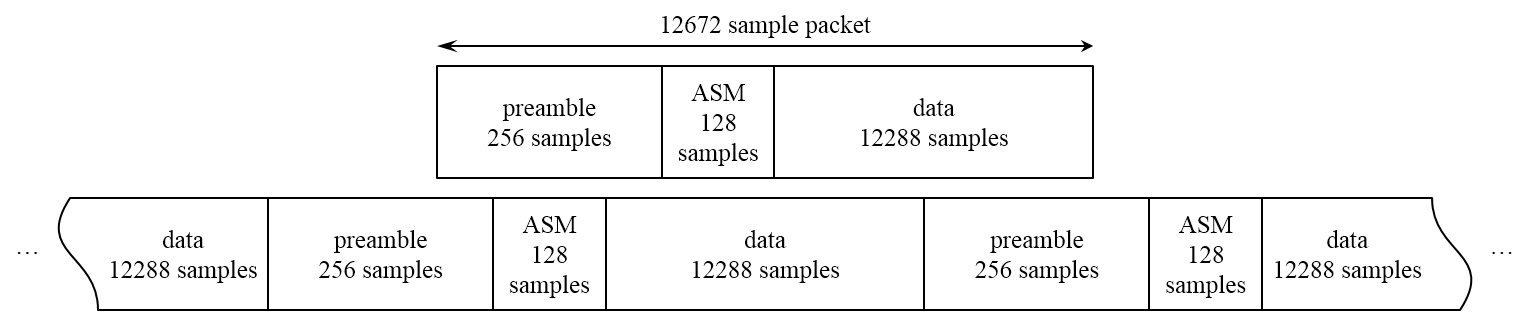
\includegraphics[width=\textwidth/10*10]{figures/gpu/packet.png}
	\caption{The iNET packet structure.}
	\label{fig:packet}
\end{figure}

To compute data-aided preamble assisted equalizers, preambles in the received signal are found then used to estimate various parameters.
The goal of the preamble detection step is to "packetize" the received samples into vectors with the packet structure shown in Figure \ref{fig:packet}. 
Each packet of received samples contains a $\Lp$ preamble samples, $\Lasm$ ASM samples and $\Ldata$ data samples.
The received signal is sampled at two samples per bit making $\Lp = 256$, $\Lasm = 136$ and $\Ldata = 12288$. 
The full length of a packet is $\Lp + \Lasm + \Ldata = 12672$.

Before the received samples can be packetized, the preambles are found using a preamble detector explained in \cite{preamble_detector}.
The preamble detector output $L(u)$ is computed by 
\begin{equation}
	L(u) = \sum_{m=0}^{7}
		\left[ I^2(n,m) + Q^2(n,m) \right]
	\label{eq:gpu-L-4}
\end{equation}
where the inner summations are
\begin{multline}
	I(n,m) \approx \sum_{\ell\in\mathcal{L}_1}r_R(\ell+32m+n)
			- \sum_{\ell\in\mathcal{L}_2}r_R(\ell+32m+n)
			+ \sum_{\ell\in\mathcal{L}_3}r_I(\ell+32m+n)
			- \sum_{\ell\in\mathcal{L}_4}r_I(\ell+32m+n)
			\\
			+ 0.7071 \left[
				\sum_{\ell\in\mathcal{L}_5}r_R(\ell+32m+n)
				- \sum_{\ell\in\mathcal{L}_6}r_R(\ell+32m+n)
			\right. \\
			\left.
				+ \sum_{\ell\in\mathcal{L}_7}r_I(\ell+32m+n)
				- \sum_{\ell\in\mathcal{L}_8}r_I(\ell+32m+n)
			\right],
	\label{eq:gpu-L-pedone-geoghegan-2}
\end{multline}
and
\begin{multline}
	Q(n,m) \approx \sum_{\ell\in\mathcal{L}_1}r_I(\ell+32m+n)
			- \sum_{\ell\in\mathcal{L}_2}r_I(\ell+32m+n)
			\\
			- \sum_{\ell\in\mathcal{L}_3}r_R(\ell+32m+n)
			+ \sum_{\ell\in\mathcal{L}_4}r_R(\ell+32m+n)
			\\
			+ 0.7071 \left[
				\sum_{\ell\in\mathcal{L}_5}r_I(\ell+32m+n)
				- \sum_{\ell\in\mathcal{L}_6}r_I(\ell+32m+n)
			\right. \\
			\left.
				- \sum_{\ell\in\mathcal{L}_7}r_R(\ell+32m+n)
				+ \sum_{\ell\in\mathcal{L}_8}r_R(\ell+32m+n)
			\right]
		\label{eq:gpu-L-pedone-geoghegan-3}
\end{multline}
with
\begin{equation}
	\begin{split}
	\mathcal{L}_1 &= \{ 0, 8, 16, 24 \}\\
	\mathcal{L}_2 &= \{ 4, 20 \}\\
	\mathcal{L}_3 &= \{ 2, 10, 14, 22 \}\\
	\mathcal{L}_4 &= \{ 6, 18, 26, 30 \}\\
	\mathcal{L}_5 &= \{ 1, 7,  9, 15, 17, 23, 25, 31 \}\\
	\mathcal{L}_6 &= \{ 3, 5, 11, 12, 13, 19, 21, 27, 28, 29 \}\\
	\mathcal{L}_7 &= \{ 1, 3,  9, 11, 12, 13, 15, 21, 23 \}\\
	\mathcal{L}_8 &= \{ 5, 7, 17, 19, 25, 27, 28, 29, 31 \}.
\end{split}
\label{eq:gpu-L-pedone-geoghegan-4}
\end{equation}
Figure \ref{fig:L_2_packets} shows $2\Lpkt$ samples of the preamble detector output $L(u)$.
\begin{figure}
	\centering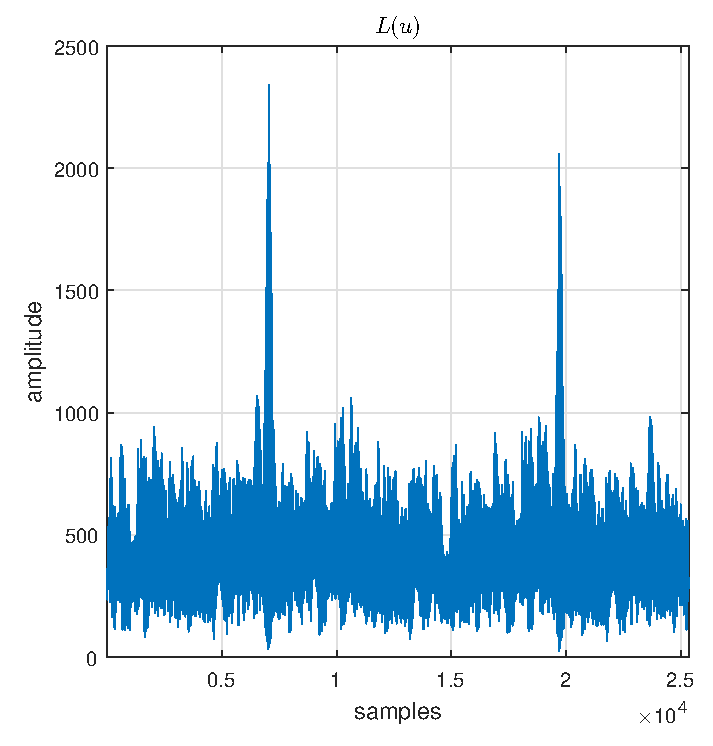
\includegraphics[width=5in]{figures/gpu/L_2_packets.eps}
	\caption{The output of the Preamble Detector $L(u)$.}
	\label{fig:L_2_packets}
\end{figure}
The start of a preamble is indicated by a local maximum of the preamble detector output.
Using the index of the local maximums, the received samples are packetized.
The vector $\rpkt$ as shown in Figure \ref{fig:simpleBlockDiagram} contains $12672$ samples of data with the packet structure shown in Figure \ref{fig:packet}.

The preamble detection algoritm in Equations \eqref{eq:gpu-L-4}-\eqref{eq:gpu-L-pedone-geoghegan-4} and the local maximum search algorithms are easily implemented into GPUs.
The GPU implementation of these algorithms wont be explained here.

\section{Frequency Offset Compensation}
\label{sec:frequency_offset_estimation_and_compensation}
The frequency offset estimator shown in Figure \ref{fig:simpleBlockDiagram} is an algorithm taken from blah.
With the notation adjusted slightly, the frequency offset estimate is
\begin{equation}
	\hat{\omega}_0 = \frac{1}{L_q} \arg\left\{ \sum_{n=i+2L_q}^{i+7L_q-1} r(n)r^\ast(n-L_q)\right\}
	\label{eq:jeff-ML-w-final3}
\end{equation}
where $L_q$ is the length of 
where a frequency offset estimate is produced for every packet in $\rpkt$.

The frequency offset is compensated for by derotating the packetized samples by $-\hat{\omega}_0$
\begin{equation}
	r(n) = r_\text{pkt}(n) e^{-j\hat{\omega}_0}
	\label{eq:frequency_compensation}
\end{equation}
Equations \eqref{eq:jeff-ML-w-final3} and \eqref{eq:frequency_compensation} are easily implemented into GPUs. 

\section{Channel Estimation}
\label{sec:channel_estimation}
The channel estimator is the ML estimator taken from blah.
\begin{equation}
\hat{\mathbf{h}} = \left( \mathbf{X}^\dag\mathbf{X} \right)^{-1} \mathbf{X}^\dag\mathbf{r}
\end{equation}
where $\mathbf{X}$ is a convolution matrix formed from the ideal preamble and ASM samples.
The matrix $\mathbf{P}_\text{ix}$ is
\begin{equation}
\mathbf{P}_\text{ix} = \left( \mathbf{X}^\dag\mathbf{X} \right)^{-1} \mathbf{X}^\dag
\end{equation}
making the channel estimate simply
\begin{equation}
\hat{\mathbf{h}} = \mathbf{P}_\text{ix} \mathbf{r}
\end{equation}
The matrix multiplication is easily implemented into GPUs.


\section{Noise Variance Estimation}
\label{sec:noise_variance_estimation}
The noise variance estimator is the algorithm taken from blah.
The algorithm is
\begin{equation}
	\hat{\sigma}_w^2 = \frac{1}{2\rho} \left| \mathbf{r}-\mathbf{X}\hat{\mathbf{h}}\right|^2
	\label{eq:ML-s2-final3}
\end{equation}
where $\rho$ is the pre-computed constant
\begin{equation}
	\rho = {\rm Trace} \left\{ \mathbf{I} -  \mathbf{X}\left(\mathbf{X}^\dag\mathbf{X}\right)^{-1}\mathbf{X}^\dag \right\}.
\end{equation}
Equation \eqref{eq:ML-s2-final3} is easily implemented into GPUs.
	

\section{SxS Detector}
\label{sec:oqpsk_detector}
The Symbol by Symbol (SxS) detector block in Figure \ref{fig:simpleBlockDiagram} is a Offset Quadtriture Phase Shift Keying (OQPSK) detector.
Using the simple OQPSK detector in place of the complex MLSE SOQPSK-TG detector leads to less than $1$ dB in bit error rate blah.
\begin{figure}
	\centering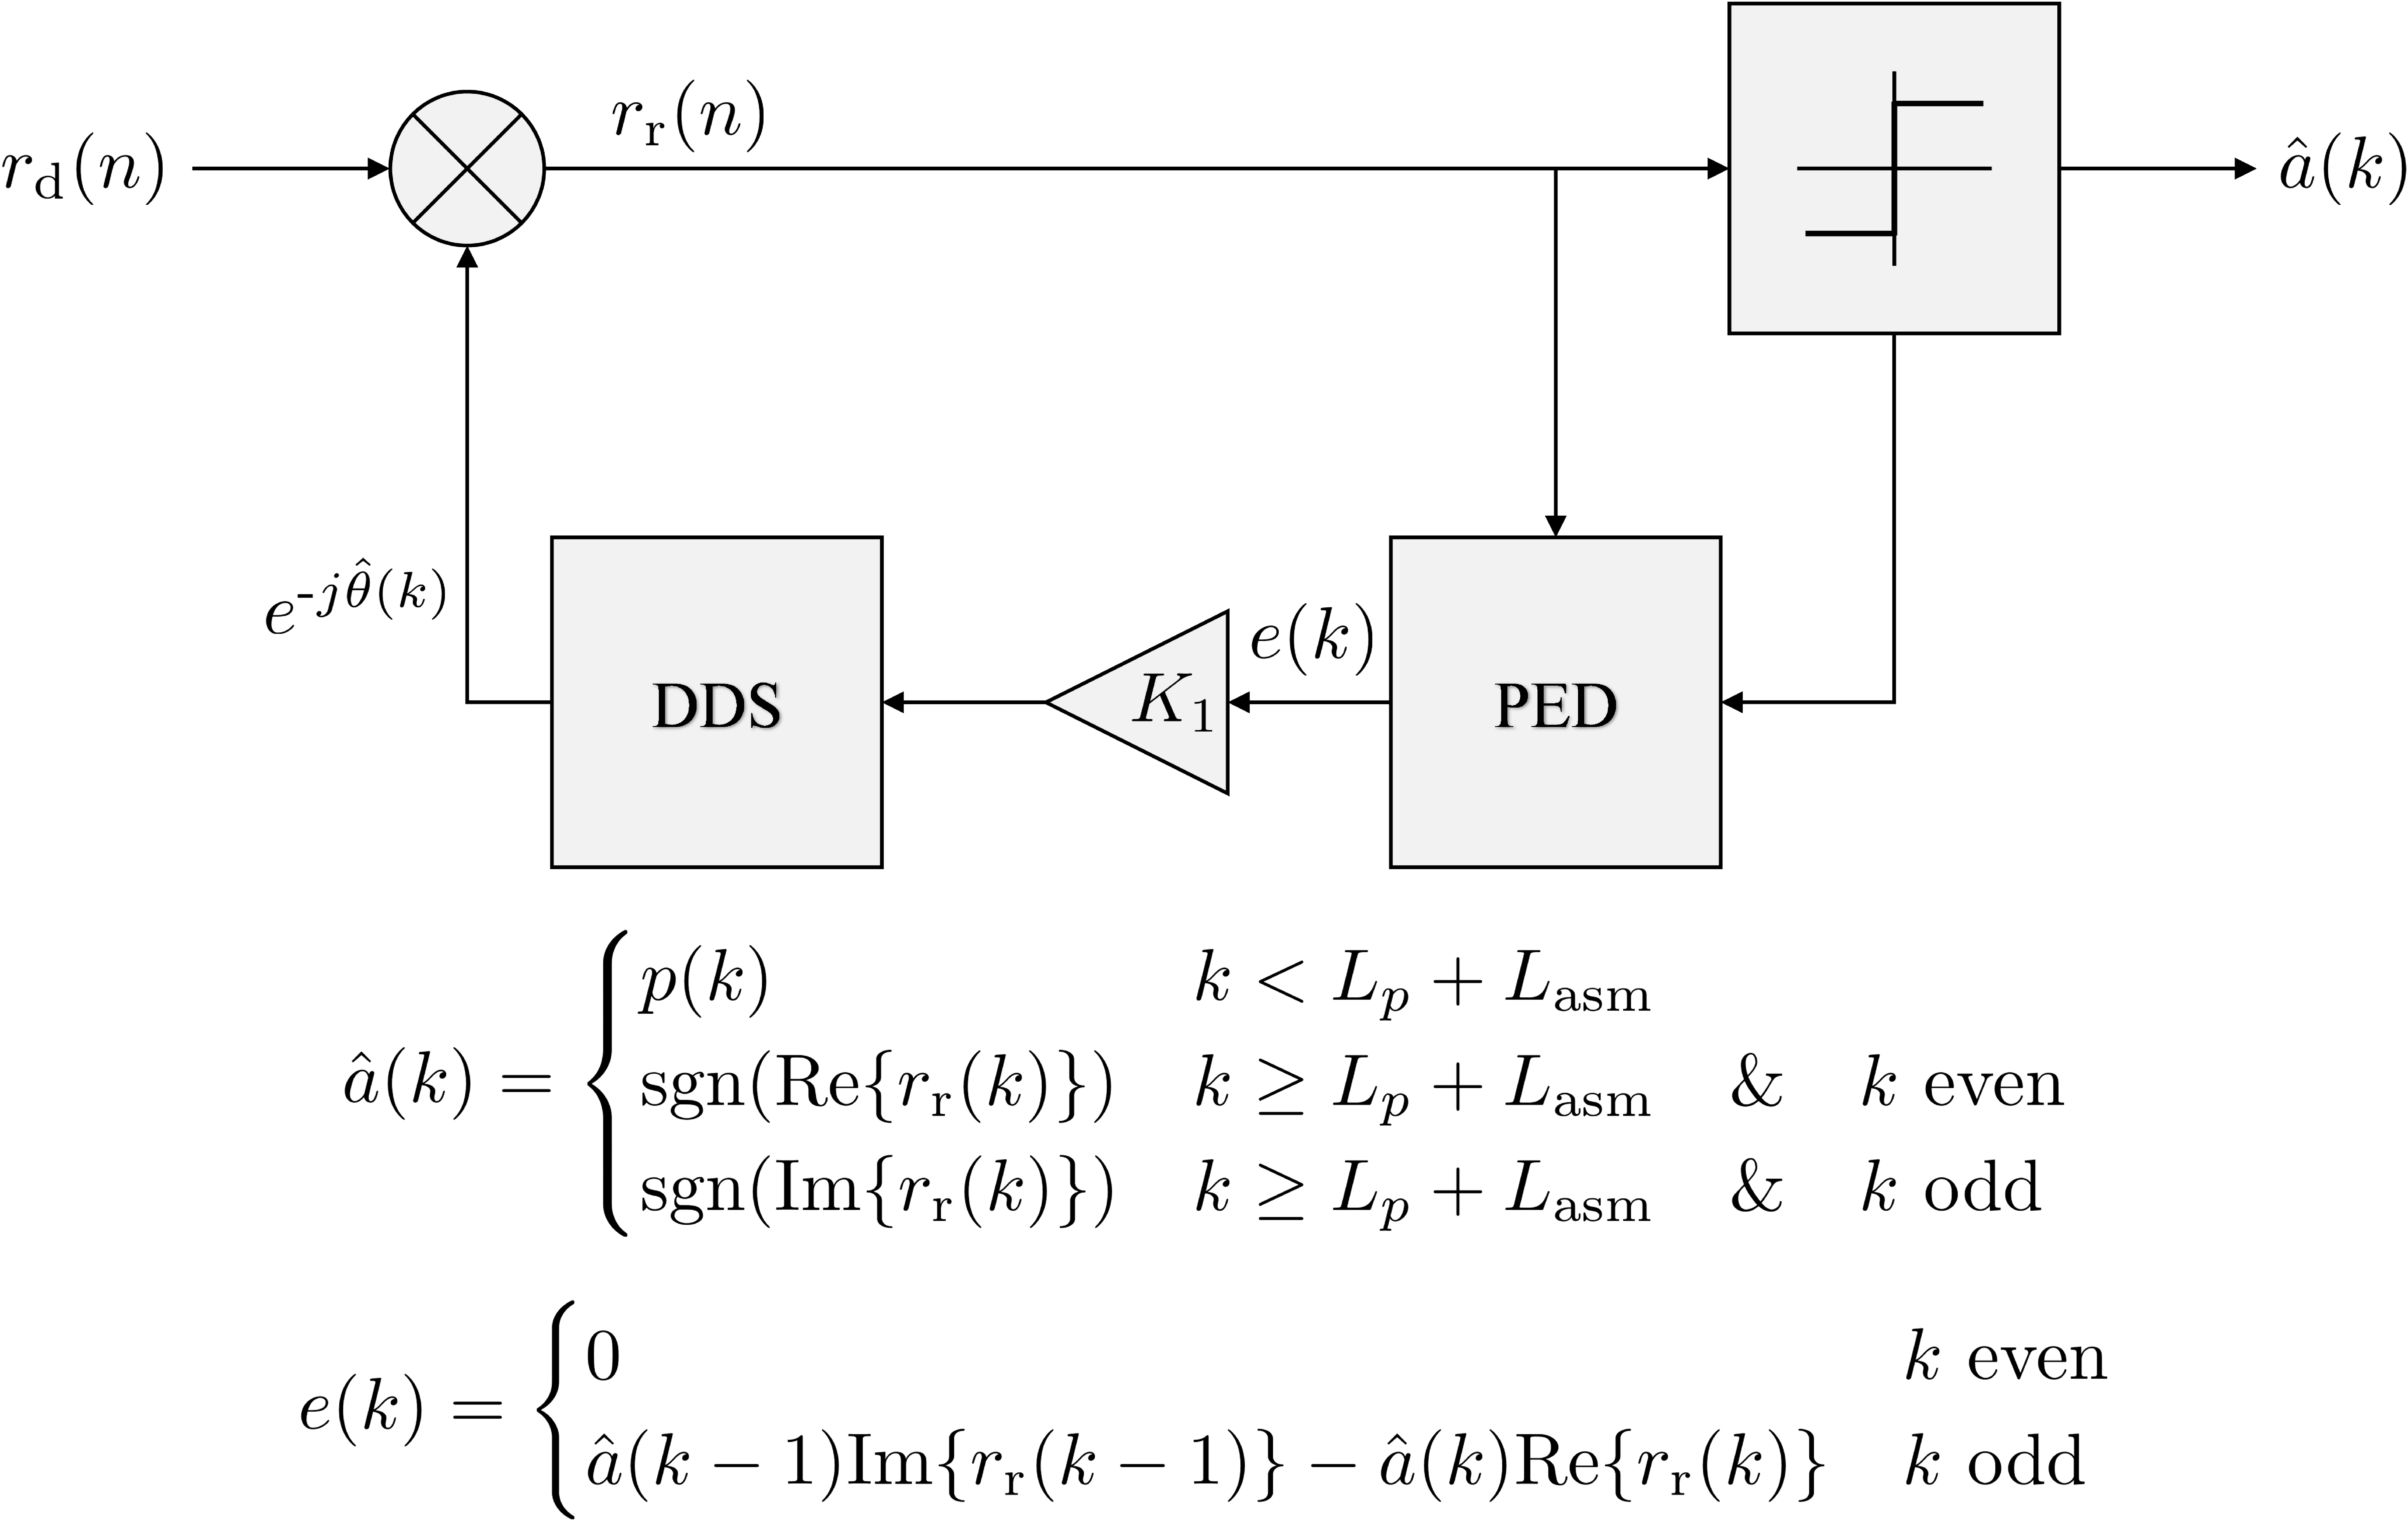
\includegraphics[width=6in]{figures/systemOverview/OQPSK.pdf}
	\caption{Offset Quadriture Phase Shift Keying symbol by symbol detector.}
	\label{fig:OQPSK}
\end{figure}

The Phase Lock Loop (PLL) in the SxS OQPSK detector cannot be parallelized to be implemented into GPUs because of the feedback loop. Feedback loops are inherently serial.
Although the OQPSK detector cannot be parallelized on a sample by sample basis, it can be parallelized on a packet by packet basis.
Running the PLL and detector serially through a full packet of data is still relatively fast because each iteration of the PLL and detector is computationally light.